\chapter{Processamento de imagens coloridas}

Capítulo 6 de Gonzalez, \textit{Digital Image Processing}~\cite{gonzalez2006image}.

\vspace{.5cm}

\begin{easylist}

  & O processamento de imagens coloridas pode ser dividido em duas grandes áreas:
  && Processamento de imagens em \textit{full-color}.
  && Processamento de imagens em cor falsa.

\end{easylist}
  
%%%%%%%%%%%%%%%%%%%%%%%%%%%%%%%%%%%%%%%%%%%%%%%%%%%%%%%%%%%%
\section{Fundamentos de teoria de cor}

\begin{easylist}

  & Percepção e interpretação: a forma como percebemos e interpretamos cores é regida por fenômenos psicofisiológicos, que envolvem estímulos dos sensores da retina e pulsos elétricos nos nervos e no córtex visual. A percepção de uma cor pode variar entre pessoas diferentes mas é determinada principalmente pela natureza da luz emitida ou refletida por um objeto.

  & Caracterização da luz: três medidas podem ser usadas para caracterizar uma fonte de luz:
  && Radiância: energia que flui de uma fonte de luz, normalmente medida em watts (W).
  && Luminância: energia que pode ser vista por um observador, medida em lumens (lm). Uma fonte de luz infravermelha pode ter muita radiância, mas terá luminância praticamente nula.
  && Brilho ou intensidade: descritor subjetivo que indica o quanto uma fonte de luz parece próxima ao branco. Uma fonte de luz verde ou amarela parece mais brilhante que uma azul ou vermelha.

  \vspace{.5cm}

  & Outra maneira de caracterizar uma fonte de luz é quanto à presença ou ausência de cor:

  && Luz acromática: é a luz sem cor. Sua única característica é a intensidade. Uma fonte de luz com todas ou algumas cores do espectro de maneira equilibrada, parecerá acromática. O termo ``tom de cinza'' se refere a uma medida escalar de intensidade que vai do preto ao branco, passando pelas diversas tonalidades de cinza.
  && Luz cromática: é a luz com cor, seja ela monocromática ou composta por vários comprimentos de onda de maneira que não pareça branca. Pode ser caracterizada pelo seu brilho, matiz e saturação. O brilho indica a noção acromática de intensidade. O matiz indica o comprimento de onda dominante, e a saturação indica se a luz é pura ou se está misturada com luz branca. As cores do espectro têm saturação máxima. As cores misturadas com branco têm pouca saturação.
  && Cromaticidade: é uma medida que une o matiz e a saturação. Portanto, uma cor pode ser caracterizada pelo seu brilho e pela sua cromaticidade. A cromaticidade é dada pela quantidade de vermelho, verde e azul que formam uma cor, e sua soma é sempre 1. 

\end{easylist}

\[ r = \frac{R}{R+G+B}
   \hspace{1.1cm}
   g = \frac{G}{R+G+B}
   \hspace{1.1cm}
   b = \frac{B}{R+G+B}
   \]

\begin{figure}[!h]
  \begin{center}
    \begin{tabular}{c}
      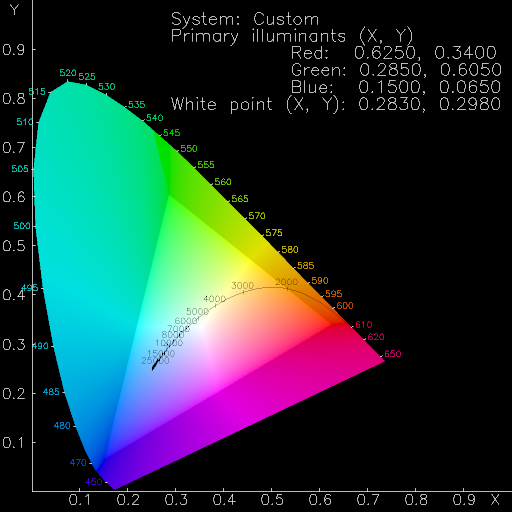
\includegraphics[width=0.7\textwidth]{images/06/chromaticity.png}
    \end{tabular}
  \end{center}
  \caption{\label{fig:chromaticity} Diagrama de cromaticidade de um certo dispositivo.}
  \source{\tt{http://www.libpng.org}.}
\end{figure}

   
%%%%%%%%%%%%%%%%%%%%%%%%%%%%%%%%%%%%%%%%%%%%%%%%%%%%%%%%%%%%
\section{Modelos de cor}

\begin{easylist}

  & Modelos de cor, também conhecidos como espaços de cor ou sistemas de cor, servem para especificar cores de maneira padronizada. É uma especificação de um sistema de coordenadas e de uma região desse espaço onde cada cor é representada por um único ponto. Geralmente, a especificação de um modelo de cor é feita para suportar algum tipo de hardware ou aplicação.

  & Tipos de modelos de cor
  && Modelos aditivos: a soma dos componentes dá branco.
  && Modelos subtrativos: a soma dos componentes dá preto.


  & Exemplos de modelos de cor
  && RGB: modelo usado para representar imagens digitais a serem exibidas em monitores. É um modelo aditivo. Consiste de três componentes: $R$, $G$ e $B$. O espaço de cor RGB costuma ser representado por um cubo de lado igual a 1. Digitalmente, cada dimensão do cubo costuma ser representada por valores de 8 bits. Dessa forma, cada pixel possui profundidade de 24 bits. Valores maiores de bits podem ser usados, caso em que temos uma imagem HDR (\textit{High Dynamic Range}). A diagonal do cubo entre os pontos $(0,0,0)$ e $(1,1,1)$ representa as escalas de cinza. O cubo completo, se representado por valores de 24 bits, é composto por $2^{24}$ cores.

\end{easylist}

  \begin{figure}[!h]
  \begin{center}
    \begin{tabular}{c}
      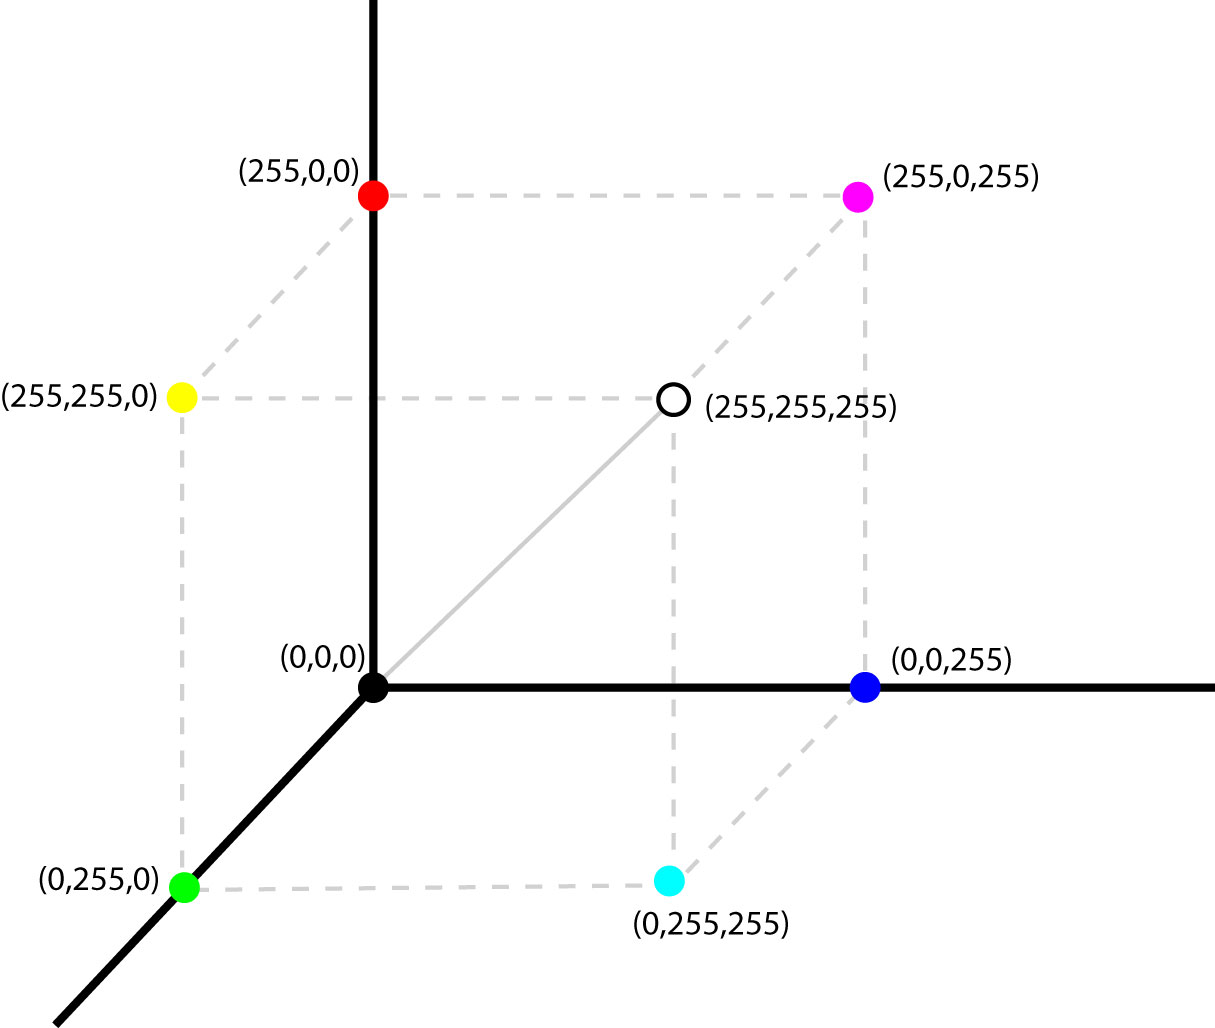
\includegraphics[width=0.5\textwidth]{images/06/RGB_cube.jpg}
    \end{tabular}
  \end{center}
  \caption{\label{fig:rgb} Espaço de cor RGB.}
  \source{\tt{http://commons.wikimedia.org}.}
\end{figure}
  
\begin{easylist}
  
  && CMY e CMYK: modelo usado por dispositivos de impressão. É um modelo subtrativo. A conversão de RGB para CMY pode ser feita através da operação:

\end{easylist}


  \[
    \begin{bmatrix}
      C \\ M \\ Y \\
    \end{bmatrix}  
    =
    \begin{bmatrix}
      1 \\ 1 \\ 1 \\
    \end{bmatrix}  
    -
    \begin{bmatrix}
      R \\ G \\ B \\
    \end{bmatrix}  
  \]

\begin{easylist}

  A cor preta é adicionada por diversas razões:

  &&& Uma impressão precisa de texto seria muito difícil sem a cor preta, pois exigiria o registro preciso dos três canais.
  &&& A composição do preto com as três cores é mais cara, requer mais tinta, pode ensopar o papel, pode demorar a secar, pode borrar a imressão, e a aparência é de uma cor escura, mas não exatamente da cor preta.

\end{easylist}
